\documentclass[UTF8, 12pt]{ctexart}
% UTF8编码,ctexart现实中文
\usepackage{color}
% 使用颜色
\usepackage{geometry}
\setcounter{tocdepth}{4}
\setcounter{secnumdepth}{4}
% 设置四级目录与标题
\geometry{papersize={21cm,29.7cm}}
% 默认大小为A4
\geometry{left=3.18cm,right=3.18cm,top=2.54cm,bottom=2.54cm}
% 默认页边距为1英尺与1.25英尺
\usepackage{indentfirst}
\setlength{\parindent}{2.45em}
% 首行缩进2个中文字符
\usepackage{setspace}
\renewcommand{\baselinestretch}{1.5}
% 1.5倍行距
\usepackage{amssymb}
% 因为所以
\usepackage{amsmath}
% 数学公式
\usepackage[colorlinks,linkcolor=black,urlcolor=blue]{hyperref}
% 超链接
\usepackage{tikz}
% 绘图
\author{Didnelpsun}
\title{多元函数积分学}
\date{}
\begin{document}
\maketitle
\pagestyle{empty}
\thispagestyle{empty}
\tableofcontents
\thispagestyle{empty}
\newpage
\pagestyle{plain}
\setcounter{page}{1}
\section{二重积分}

\subsection{交换积分次序}

\subsubsection{直角坐标系}

\textbf{例题:}交换积分次序$\int_0^1\textrm{d}x\int_0^{x^2}f(x,y)\,\textrm{d}y+\int_1^3\textrm{d}x\int_0^{\frac{1}{2}(3-x)}f(x,y)\,\textrm{d}y$。

解:已知积分区域分为两个部分。将$X$型变为$Y$型。画出图形可以知道$y\in(0,1)$,$x$的上下限由$y=x^2$和$y=\dfrac{1}{2}(3-x)$转化为$\sqrt{y}$和$3-2y$。

所以转换为$\int_0^1\textrm{d}y\int_{\sqrt{y}}^{3-2y}f(x,y)\,\textrm{d}x$。

\subsubsection{极坐标系}

\textbf{例题:}对$\int_{-\frac{\pi}{4}}^{\frac{\pi}{2}}\textrm{d}\theta\int_0^{2\cos\theta}f(r\cos\theta,r\sin\theta)r\,\textrm{d}r$交换积分次序。

解:对于极坐标的积分次序交换需要利用直角坐标系来画图了解,特别是对于$r$的上下限。

对$\theta=\dfrac{\pi}{2}$变为$y$轴,$y=-\dfrac{\pi}{4}$变为$y=-x$。

对$r=2\cos\theta$变为$xy$的表达式,$r^2=2\cos\theta$,即$x^2+y^2=2x$,$(x-1)^2+y^2=1$。

\begin{minipage}{0.625\linewidth}
    所以所得到的$\sigma$为一个圆割去一个扇形。
    
    交换积分次序后就需要以一个长度以极点为圆心做圆,切割$\sigma$。

    由$\sigma$可知取长度$\sqrt{2}$可以切分。
\end{minipage}
\hfill
\begin{minipage}{0.25\linewidth}
    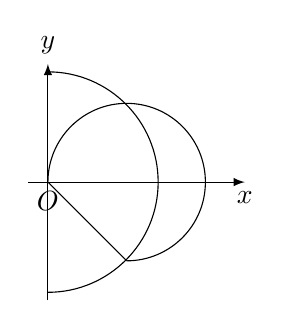
\begin{tikzpicture}[scale=1]
        \draw[-latex](-0.25,0) -- (2.5,0) node[below]{$x$};
        \draw[-latex](0,-1.5) -- (0,1.5) node[above]{$y$};
        \filldraw[black] (0,0) node[below]{$O$};
        \draw (1,-1) arc (-90:180:1);
        \draw (0,0) -- (1,-1);
        \draw (0,-1.4) arc (-90:90:1.4);
    \end{tikzpicture}
\end{minipage}

所以$\sigma$可以分为左边的$\sigma_1$和右边的$\sigma_2$。

$\sigma_1$的$r\in[0,\sqrt{2}]$,$\sigma_2$的$r\in[\sqrt{2},2]$。

$\sigma_1$的$\theta$下限是$y=-x$这条边,即$\theta=-\dfrac{\pi}{4}$,上限是$r=2\cos\theta$这个圆,则$\theta=\arccos\dfrac{r}{2}$。

$\sigma_2$的$\theta$界限都是是$r=2\cos\theta$这个圆,此时$r>0$恒成立,但是上限是上半部分$\theta>0$,而下限是下半部分$\theta<0$,即上限$\theta=\arccos\dfrac{r}{2}$,所以下限为$\theta=-\arccos\dfrac{r}{2}$。

综上交换积分次序结果为:

$\int_0^{\sqrt{2}}r\,\textrm{d}r\int_{-\frac{\pi}{4}}^{\arccos\frac{r}{2}}f(r\cos\theta,r\sin\theta)\textrm{d}\theta+\int_{\sqrt{2}}^2r\,\textrm{d}r\int_{-\arccos\frac{r}{2}}^{\arccos\frac{r}{2}}f(r\cos\theta,r\sin\theta)\textrm{d}\theta$。

\subsection{极直互化}

\textbf{例题:}将$I=\int_0^{\frac{\sqrt{2}}{2}R}e^{-y^2}\textrm{d}y\int_0^ye^{-x^2}\,\textrm{d}x+\int_{\frac{\sqrt{2}}{2}R}^Re^{-y^2}\,\textrm{d}y\int_0^{\sqrt{R^2-y^2}}e^{-x^2}\,\textrm{d}x$转换为极坐标系并计算结果。

解:首先根据积分上下限得到积分区域$D=\left\{0\leqslant y\leqslant\dfrac{\sqrt{2}}{2}R,0\leqslant x\leqslant y\right\}\cup\left\{\dfrac{\sqrt{2}}{2}R\leqslant y\leqslant R,0\leqslant x\leqslant\sqrt{R^2-y^2}\right\}$,$D$为一个八分之一圆的扇形。

根据$x=r\cos\theta$,$y=r\sin\theta$替换得到$D=\left\{(x,y)\bigg|0\leqslant r\leqslant R,\dfrac{\pi}{4}\leqslant\theta\leqslant\dfrac{\pi}{2}\right\}$。

又$e^{-y^2}\cdot e^{-x^2}=e^{-(x^2+y^2)}=e^{-r^2}$。

$\therefore I=\int_{\frac{\pi}{4}}^{\frac{\pi}{2}}\textrm{d}\theta\int_0^Re^{-r^2}r\,\textrm{d}r$。

\subsection{二重积分计算}

二重积分若是累次积分形式出现,则计算可以使用上面两种方法简便运算。

\subsubsection{交换积分次序}

当按照当前的积分次序无法算出时需要更换积分次序。主要是看$f(x,y)$是对$x$先积分更简单还是对$y$先积分更简单。

\textbf{例题:}求$\int_0^1\textrm{d}y\int_{\arcsin y}^{\pi-\arcsin y}\cos^2x\,\textrm{d}x$。

解:首先直接对这个式子直接计算,$\cos^2x=\dfrac{1}{2}(1+\cos2x)$,原式$=\dfrac{1}{2}\int_0^1(\pi-2y-\arcsin y)\textrm{d}y$。根本无法解出。

考虑交换积分次序,首先求$\sigma$,$y\in[0,1]$,$x\in[\arcsin y,\pi-\arcsin y]$,则$\sin x=y$,$y=\sin(\pi-x)=\sin x$即$x\in[0,\sin x]$。

将积分区域换成$X$型:$x\in[0,\pi]$,$y\in[0,\sin x]$。

$\int_0^\pi\cos^2x\,\textrm{d}x\int_0^{\sin x}\textrm{d}y=\int_0^\pi\cos^2x\sin x\,\textrm{d}x=-\int_0^\pi\cos^2x\,\textrm{d}(\cos x)=-\dfrac{\cos^3x}{3}\bigg|_0^\pi\\=\dfrac{2}{3}$。

\subsubsection{积分性质}

若积分区域$\sigma$关于$x=k_1$或$y=k_2$对称,则当$f(x,y)$含有$x-k_1$或$y-k_2$因式时重积分值为0。

\textbf{例题:}设$D:x^2+y^2\leqslant2x+2y$,求$\iint\limits_Dxy\,\textrm{d}x\textrm{d}y$。

解:本题目使用直角坐标系和极坐标系都不好做。所以需要利用积分性质,对$D$进行平移等操作。

利用平移,由于$D:(x-1)^2+(y-1)^2=2$,令$x=1+r\cos\theta$,$y=1+r\sin\theta$,则利用极坐标,$r\in[0,\sqrt{2}]$,$\theta\in[0,2\pi]$,$=\int_0^{2\pi}\textrm{d}\theta\int_0^{\sqrt{2}}((1+r\cos\theta)(1+r\sin\theta)r)\textrm{d}r=\int_0^{2\pi}\textrm{d}\theta\int_0^{\sqrt{2}}(1+r\sin\theta+r\cos\theta+r^2\sin\theta\cos\theta)r\,\textrm{d}r$,又将$\sin\theta$和$\cos\theta$对$\theta$在$[0,2\pi]$进行积分全部为0,所以直接把后面的全消掉,变为$\int_0^{2\pi}\textrm{d}\theta\int_0^{\sqrt{2}}r\,\textrm{d}r=2\pi$。

\subsubsection{切分区域}

\textbf{例题:}设$D=\{(x,y)|0\leqslant x\leqslant1,0\leqslant y\leqslant1\}$,求$\displaystyle{\iint\limits_D\dfrac{\textrm{d}x\textrm{d}y}{\sqrt{x^2+y^2}}}$。

解:由$f(x,y)=\dfrac{1}{\sqrt{x^2+y^2}}$,知道可以使用极坐标系来表示,但是$D$是一个正方形,无法用圆来简单表示。

又$D$可以从$y=x$切割为两个部分,所以令下三角形为$D_1$,$\displaystyle{\iint\limits_D\dfrac{\textrm{d}x\textrm{d}y}{\sqrt{x^2+y^2}}}=2\displaystyle{\iint\limits_{D_1}\dfrac{\textrm{d}x\textrm{d}y}{\sqrt{x^2+y^2}}}$。

所以$0\leqslant y$和$y=x$可以确定$\theta\in\left[0,\dfrac{\pi}{4}\right]$,$0\leqslant x\leqslant1$可以确定$r$上界为$x=1$,即$r\cos\theta=1$,即$r=\dfrac{1}{\cos\theta}$,确定$r\in\left[0,\dfrac{1}{\cos\theta}\right]$。

所以$=2\int_0^{\frac{\pi}{4}}\textrm{d}\theta\int_0^{\frac{1}{\cos\theta}}\textrm{d}r=2\int_0^{\frac{\pi}{4}}\dfrac{\textrm{d}\theta}{\cos\theta}=2\ln(\sec\theta+\tan\theta)|_0^{\frac{\pi}{4}}=2\ln(1+\sqrt{2})$。

\end{document}
